\section{Motivating Examples}
\label{sec:examples}

In section~\ref{sec:method}, we presented a framework for constructing
an ROS (if deemed advantageous) by identifying unimportant parameters based on 
estimates of the screening metric, $\widehat{\mathcal{C}_i\mu_i}$
for individual parameters.
In this section, we motivate the underlying methodology by applying it to three test problems,
namely, the borehole function, a non-linear oscillator, and a semi-linear elliptic PDE.
Since model evaluations in all these test
problems are inexpensive, we compare relative importance of model parameters based
on the screening metric, obtained using model evaluations with 
converged estimates of $\mathcal{T}(\theta_i)$ based on the surrogate constructed in the
full parameter space (FSS). Additionally, to illustrate computational gains, we compare
convergence trends as a function of training runs for the ROS and the FSS using 
$\epsilon_{\mbox{\tiny LOO}}$ in Eq.~\ref{eq:loo}. 
Furthermore, as discussed earlier in section~\ref{sec:method}, we compare
PDFs of the model output, obtained using the ROS and the full-space surrogate for
the purpose of verification. 

\subsection{Borehole function}

The borehole function is a benchmark reference problem in sensitivity analysis. It models the discharge
of water ($\mathcal{Q}$) through a borehole in terms of geometrical and physical parameters:

\be
\mathcal{Q} = \frac{2\pi T_u(H_u - H_l)}{\ln\left(\frac{r}{r_w}\right)\left(1 +
\frac{2LT_u}{\ln\left(\frac{r}{r_w}\right)r_w^2K_w} + \frac{T_u}{T_l}\right)}
\label{eq:bore}
\ee

\noindent The radius of influence, $r$ is fixed at 3698.30 m whereas all other parameters
in the right hand side of~\eqref{eq:bore} are considered 
as uncertain. Thus, $\mathcal{Q} = \mathcal{Q}(\vec{\theta})$ with 
\[
   \vec{\theta} = (r_w, L, T_u, H_u, T_l, H_l, K_w)^T.
\] 
Table~\ref{tab:bore} provides distributions of the uncertain inputparameters. 

\begin{table}[htbp]
\renewcommand*{\arraystretch}{1.2}
\begin{center}
\begin{tabular}{|c|c|}
\hline
Parameter & Distribution \\ \hline \hline
$r_w$ (Borehole radius, m) & $\mathcal{N}$(0.1,0.016) \\
$L$ (Borehole length, m) & $\mathcal{U}$[1120,1680] \\
$T_u$ (Transmissivity of upper aquifer, m$^2$/yr) & $\mathcal{U}$[63070,115600] \\
$H_u$ (Potentiometric head of upper aquifer, m) & $\mathcal{U}$[990,1110] \\
$T_l$ (Transmissivity of lower aquifer, m$^2$/yr) & $\mathcal{U}$[63.1,116] \\
$H_l$ (Potentiometric head of lower aquifer, m) & $\mathcal{U}$[700,820] \\
$K_w$ (Borehole hydraulic conductivity, m/yr) & $\mathcal{U}$[9855,12045] \\
\hline
\end{tabular}
\end{center}

\caption{Description and distributions of uncertain parameters in the borehole function
given by~\eqref{eq:bore}.}
\label{tab:bore}
\end{table}

Cheap function evaluations of the discharge $\mathcal{Q}(\vec{\theta})$ using
enables computing accurate estimates of $\mathcal{T}(\theta_i)$ through
sampling, with a sufficiently large Monte Carlo sample size.  Shown in
Figure~\ref{fig:sense_bore}~(left) are estimates of these indices corresponding to the
uncertain parameters in the borehole function using 10$^6$ pseudo-random
samples in the input parameter space. 
%\footnote{Although $\mathcal{T}(\theta_i)$ might converge with much fewer
%samples depending upon the model, we consider a large number that typically
%ensures a converged estimate for the purpose of illustration.} 
These estimates are used to verify fidelity of
parameter screening based on the methodology presented in Section~\ref{sec:method}. 

\begin{figure}[htbp]
 \begin{center}
  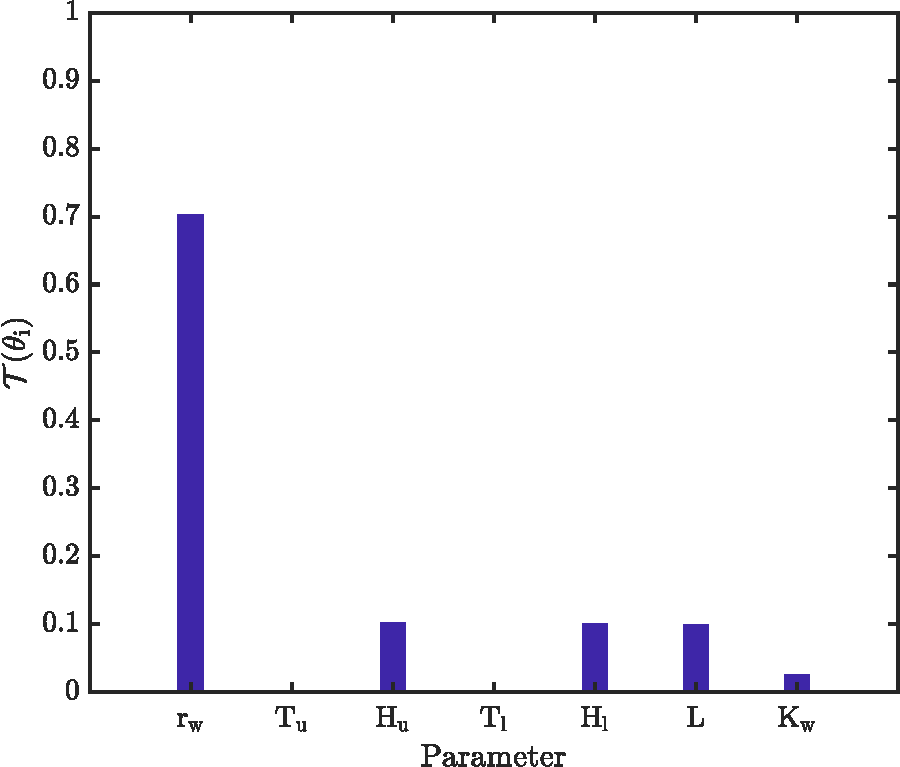
\includegraphics[width=0.48\textwidth]{./Figures/sense_borehole}
  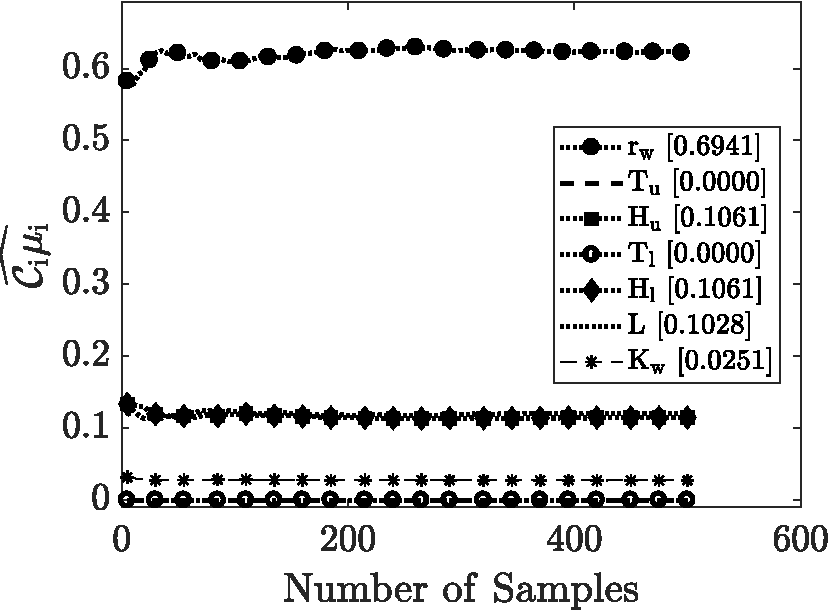
\includegraphics[width=0.51\textwidth]{./Figures/ub_conv_borehole}
\caption{
Left: Sobol' total sensitivity index for uncertain parameters in the borehole
function. Right: 
estimates of the screening parameter ($\widehat{\mathcal{C}_i\mu_i}$) is plotted
against number of samples considered for evaluating $\mu_i$. Corresponding estimates
for the converged Sobol' total effect index ($\mathcal{T}(\theta_i)$) in each case is also included in the
legend. }
\label{fig:sense_bore}
\end{center}
\end{figure}
In Figure~\ref{fig:sense_bore}~(right), we plot estimates of the screening parameter 
$\widehat{\mathcal{C}_i\mu_i}$ for a wide range of the number of 
samples used for approximating $\mu_i$ using~\eqref{eq:mu}.
Estimates for $\widehat{\mathcal{C}_i\mu_i}$ are found to be in excellent agreement
with $\mathcal{T}(\theta_i)$ even when small number of samples (5--10) are used. 
Consequently, the relative importance of uncertain 
parameters in the borehole function is found to be consistent 
with predictions based on the Sobol' index. 
In the considered intervals for the uncertain parameters, it is clear 
that the discharge is insensitive to $T_u$ and $T_l$. 
Moreover, the sensitivity to $K_w$ is also small. We exploit these findings to reduce
the dimensionality of the problem by 
discounting the uncertainties in $T_u$, $T_l$, and $K_w$ by fixing 
them at their respective nominal values. 

Our goal as discussed is to gain computational advantage by constructing
surrogates in a reduced input parameter space. To this end, we use LAR to 
construct PCEs
in 5D and 4D spaces by fixing $\{T_u,T_l\}$ in the former and additionally
fixing $K_w$ in the latter at their respective mean values. In
Figure~\ref{fig:conv_bore}(left), we compare convergence of PCEs constructed in the
full space (7D) with those constructed in the two reduced spaces (4D and 5D)
using $\epsilon_{\mbox{\tiny{LOO}}}$ (Eq.~\ref{eq:loo}). 

\begin{figure}[htbp]
 \begin{center}
  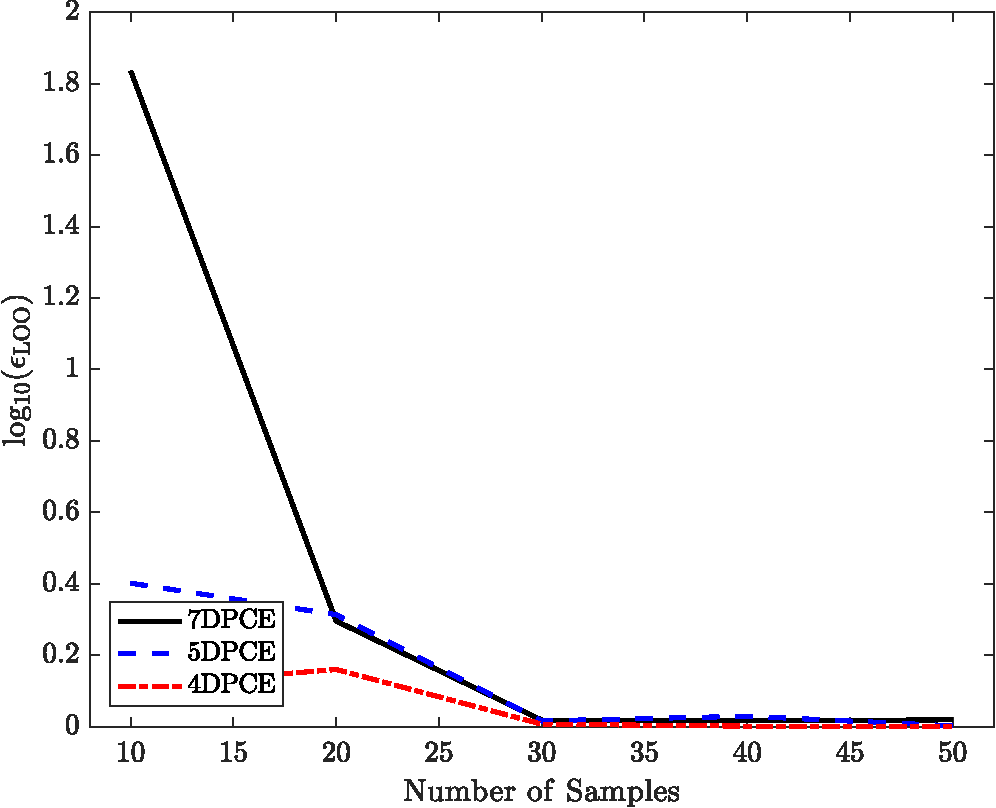
\includegraphics[width=0.48\textwidth]{./Figures/err_samples_borehole}
  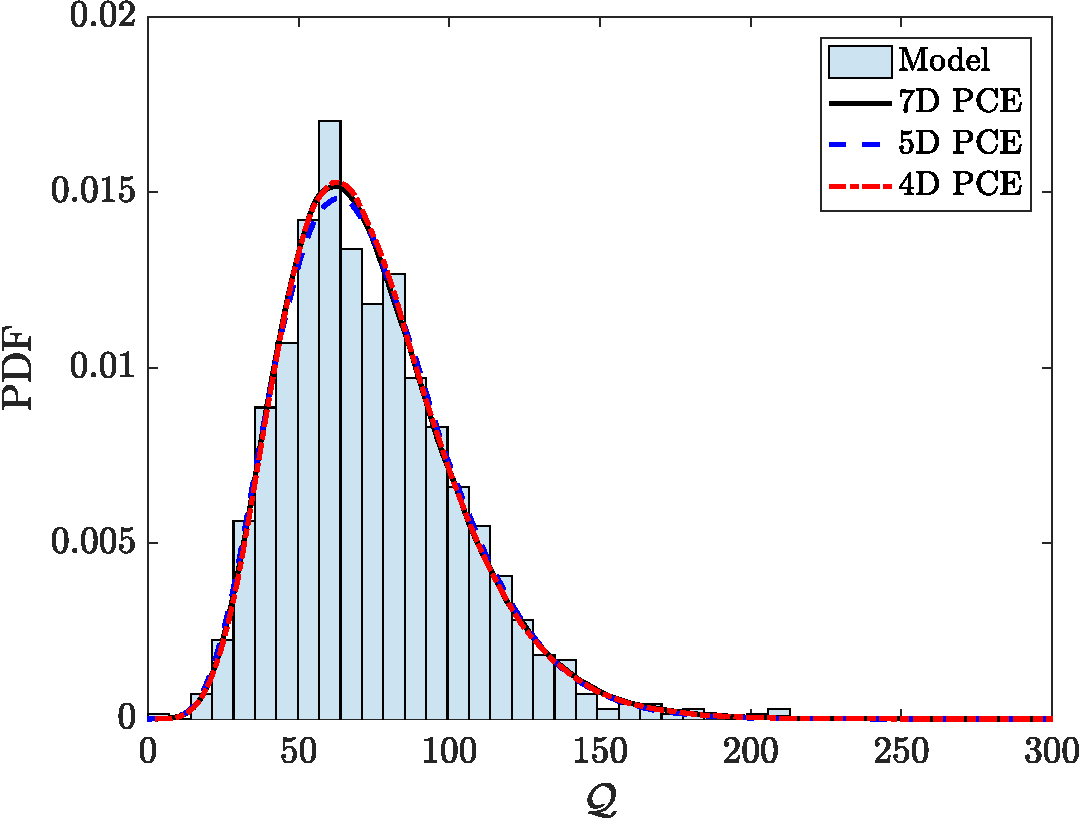
\includegraphics[width=0.48\textwidth]{./Figures/pdf_comp_borehole}
\caption{Left: A comparison of order of the leave-one-out-error 
($\epsilon_{\mbox{\tiny{LOO}}}$) as a function of number of regression samples
used for constructing the PCE in 4, 5, and 7 dimensions. Right: A comparison of
PDFs of the discharge, $\mathcal{Q}$, generated using 10$^{6}$ samples from
the marginal distributions of the uncertain parameters in each case.} 
\label{fig:conv_bore}
\end{center}
\end{figure}

As expected, it is observed that the PCE constructed in the 4D space converges
at a much faster rate. For instance, if a PCE with $\mathcal{O}(10^{-4})$
accuracy is sought, we need function evaluations at only about 50 sample points
in the 4D parameter space whereas the number of samples needed in the full 7D
space seems much higher. Latin hypercube sampling (LHS) was used in
each case. It must be pointed out that the error in Figure~\ref{fig:conv_bore}(left)
is not expected to decrease monotonically with the increase in sample size
owing to the penalty term in the regularized optimization problem in Eq.~\ref{eq:reg}. 


As discussed earlier in this section, the reduced order PCE's are verified for
predictive accuracy in a least-squares sense and a probabilistic sense.
Estimates for $\epsilon_{\mbox{\tiny{L-2}}}$ based on 50 samples and
corresponding function evaluations in the original 7D parameter space were
found to be 0.0551 and 0.0112 for the 4D and 5D PCE's respectively. In other
words, the 4D PCE is accurate within 5.52$\%$ and the 5D PCE is accurate within
1.12$\%$ of predictions based on the borehole function. We note  that although
the convergence in the case of a 5D PCE is slower (Figure~\ref{fig:conv_bore}),
its predictive accuracy is higher than the 4D PCE. This illustrates the
tradeoff between accuracy and computational efficiency for the present 
problem. Generally, the required level of accuracy is problem dependent. 
The present framework allows for moving towards higher fidelity 
reduced order surrogates based on the ranking of the parameter sensitivities. 
 
%A possible explanation for this observation is that above a certain order
%of convergence, the uncertainty in $k_w$ contributes much more towards
%predictive accuracy of the reduced order PCE. It is therefore critical to
%account for the order of PCE convergence as well as its predictive accuracy for
%a given application, as highlighted earlier in section~\ref{sec:method}. 


Figure~\ref{fig:conv_bore}(right) illustrates a comparison of the PDFs
of the
discharge, $\mathcal{Q}$ obtained by propagating 10$^6$ random
samples through the 7D PCE in the original input parameter domain as well as
the reduced order PCEs constructed in 4 and 5 dimensions. 
It is evident from this plot, that the PDFs agree quite favorably with each
other with respect to the modal estimate as well as the uncertainty associated with 
$\mathcal{Q}$. 
Consequently, it can be said that the reduced order PCE is verified in a
probabilistic sense. In other words, the mode as well as the uncertainty in the
observable is reliably captured and predicted by the reduced order PCE. 
 
\subsection{Non-linear Oscillator}

\subsection{Semilinear elliptic PDE with random source term}

We consider the semilinear elliptic PDE,
\begin{equation}\label{equ:semilinear}
\begin{aligned}
-\kappa \Delta u + c u^3 &= q, \quad \text{in } \Omega\\
 u &= 0. \quad \text{on } \partial \Omega
\end{aligned}
\end{equation}
We model the source term as 
\begin{equation}
q(x, y, \theta) = \sum_{i = 1}^N \theta_i \sin(i \pi x)
\cos(i \pi y),
\quad N = 8.
\end{equation}
Here $\kappa \sim U(0.08, 0.12)$, $c \sim U(0.8, 1.2)$, 
and $\theta_i$ are uniformly distributed in interval $[0, 1]$. We consider
the following QoI,
\[
     f(\kappa, c, \theta) = \frac{1}{|D|} \int_D u(x; \kappa, c, \theta) \, dx, 
\]
where $D$ is the region, $[1/2, 3/4] \times [1/2, 3/4]$.

































